\documentclass[tikz]{standalone}
\usetikzlibrary{calc}
\usepackage{pgfplots}
\usepgfplotslibrary{polar}
\pgfplotsset{compat=1.9}

\usepackage{amsmath}

\begin{document}

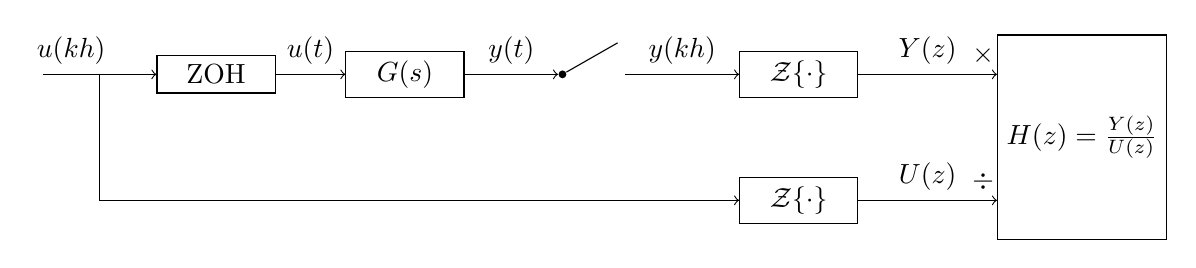
\begin{tikzpicture}[node distance=20mm, block/.style={rectangle, draw, minimum width=15mm, }]

\node[coordinate] (input) {};
\node[block, right of=input, node distance=22mm] (zoh) {ZOH};
\node[block, right of=zoh, node distance=24mm] (G) {$G(s)$};
\node[circle, fill, inner sep=1pt, right of=G] (sampleyin) {}; 
\node[coordinate, right of=sampleyin, node distance=8mm] (sampleyout) {}; 
\node[block, right of=sampleyout, node distance=22mm] (ztrfY) {$\mathcal{Z}\{\cdot \}$}; 
\node[coordinate, below of=ztrfY, node distance=8mm] (ztrfmid) {};
\node[block, below of=ztrfmid, node distance=8mm] (ztrfU) {$\mathcal{Z}\{\cdot \}$}; 
\node[coordinate, right of=ztrfmid, node distance=36mm] (Hztmp) {};
\node[block, minimum height=26mm, above of=Hztmp, node distance=0mm] (Hz) {$H(z)=\frac{Y(z)}{U(z)}$};

\draw[->] (input) -- node[coordinate] (measureu) {} node[above,near start] {$u(kh)$} (zoh);
\draw[->] (zoh) --  node[above] {$u(t)$} (G);
\draw[->] (G) -- node[above] {$y(t)$} (sampleyin);
\draw (sampleyin) -- ++(7mm,4mm);
\draw[->] (sampleyout) -- node[above] {$y(kh)$} (ztrfY);
\draw[->] (measureu) |- (ztrfU);
\draw[->] (ztrfU) -- node[above] {$U(z)$} node [above, pos=0.9] {$\div$} (ztrfU -| Hz.west);
\draw[->] (ztrfY) -- node[above] {$Y(z)$} node [above, pos=0.9] {$\times$} (ztrfY -| Hz.west);

\end{tikzpicture}
\end{document}
